%!TEX root = ../../super_main.tex
\part{Fourth Sprint}
\label{par:fourth_sprint}

\chapter{Sprint Overview}
In the fourth sprint, our group asked for a role, dubbed ``\giraf Police'', which included the responsibility of \gc and the responsibility to make sure the other groups implemented \gc as they should. We also decided to synthesize a design manual from all our thoughts of the design of \giraf and our attempts to unify the overall design throughout the project in order to pass our design ideas on to the next semesters. The design manual can be found in \appref{app:design_manual}. We were also tasked with further polishing and maintenance of the \ct and the \launcher. 
\\\\
The customers was for the last time asked to prioritize the applications. \figref{tab:application_priorities_sprint_four} shows how the customers have prioritized the different applications for the fourth sprint.

\begin{table}[!htbp]
	\center
    \begin{tabular}{l l}
        \textbf{Application}     & \textbf{Priority} \\ \hline\hline
        \launcher                & 0                 \\ \hline
        \gc         		     & 0                 \\ \hline
        \emph{Picto Creator}     & 1                 \\ \hline
        \ct                      & 2                 \\ \hline
        \emph{Sequence}          & 3                 \\ \hline
        \emph{Week Schedule}     & 4                 \\ \hline
        \emph{Profile Manager}   & 5                 \\ \hline
        \emph{Picto Search}      & 6                 \\ \hline
        \emph{Picto Reader}      & 7                 \\ \hline
        \emph{Web admin}         & 8                 \\ \hline
        \emph{Category Game}     & 9                 \\ \hline
        \emph{Timer}             & 10                \\ \hline
        \emph{Life Story}        & 11                \\ \hline
        \emph{Voice Game}        & 12                \\ \hline
    \end{tabular}
    \caption{Application priorities}
    \label{tab:application_priorities_sprint_four}
\end{table}

\FloatBarrier

%!TEX root = ../../../super_main.tex

\chapter{Design Manual}
\label{cha:design_manual}

Throughout the fourth sprint, development of the design manual had a high priority for our group. Roughly half of the group's resources were used on the development of the manual. From the start, we knew that we would not be able to complete the manual \todo{write why, workload, unconsidered design decisions etc.}, so we focused a lot on getting already agreed-upon design guides formalized. This chapter will describe the development of the manual. The latest version of the design manual can be found in \appref{app:design_manual}.

\section{Development}
\label{sec:development}
\todo[inline]{More fixed by niklas START} In the third sprint, a GUI design-meeting was arranged to ensure that new and previous GUI-groups all agreed on the same design principles \todo{skriv at der kom flere gui grupper og de skulle lige håndtere vores aftaler}. \todo[inline]{More fixed by niklas END} The results of this meeting were meant to be implemented in the former design guidelines made by group \emph{SW606F15}. However, this was only documented on a note basis, and would not be instructive to new \giraf developers about the design. Because of this, it was prioritized to get these notes formalized and described in details in the new design manual. The previous design guide can, as previously mentioned, be found in their report\footnote{This report has not yet been published, and we are therefore unable to cite it properly}.

\section{Complying with the Manual}
\label{sec:complying_with_the_manual}
While developing the manual, we looked at the different applications in the \giraf software suite to see if we could help other groups with improving the design of their applications so that their applications could become more usable and more consistent with the other applications. After checking the different applications, we sat down with members from the various groups and gave them a walk-through of the issues we found, such that they had time to correct the issues or document them properly before the Sprint Review Meeting.
\\\\
While looking through the different applications, we found some design cases that were not considered in the developed design manual. Due to limited time in the fourth sprint, it was decided not to write additional sections in the manual to cover these cases. Instead of just deciding upon the design in these cases for ourself, we have written notes throughout the design-manual to indicate where the design is incomplete or needs attention. These notes describe the different choices that the next generation of \giraf developers will have to consider in order to complete the manual. Ideally, the groups next semester should have a meeting between all GUI-groups to discuss how design issues should be resolved.

%!TEX root = ../../../super_main.tex
\chapter{Issues and Solutions}
\label{cha:issues_and_solutions}

\todo[inline]{Insert introduction to the chapter}

%!TEX root = ../../../super_main.tex

\section{Deprecation of Old Code}
\label{sec:deprecation_of_old_code}

As part of the further development of \gc we decided to deprecate and eventually remove a lot of old, unused, and unstable classes from the previous semesters. This is something we decided to do in order to force the other developers to use our newly developed components, since we found that people were hesitant to change components if it was not necessary.\\

We started the process by deprecating most of the classes that had been replaced, along with those we found unused. After a while, we notified the other GUI groups via email, that we intended to release a new major version of the \gc library without these deprecated classes in a near future. A few days later we did as promised - deleted the classes and shipped the new version. 

%!TEX root = ../../../super_main.tex

\section{\emph{Launcher} Sessions}
\label{sec:launcher_session_issues}

The \launcher had a problem with its user sessions, where it was impossible to login with a guardian profile, once a citizen profile had logged in. The only way of logging back into a guardian account was to terminate and restart the application.
\\\\
The problem was caused by the fact that the \androidinline{HomeActivity} from the previous session was reused by the Android system, when the user had logged out and started a new session with a new login.
\\\\
The solution is to force the system to create a new \androidinline{HomeActivity} for any new session, by applying a flag to the \androidinline{Intent} used to start the new \androidinline{HomeActivity}. At the same time, we also added a flag to all activities in the \launcher that ensures that only one instance of the different activities can be active at any one time. This ensures that any old instances of a given subclass of \androidinline{Activity} would be removed before a new one is added to \launcher's stack of \androidinline{Activity} objects and there is therefore no danger of automatic reuse of any old version of the same \androidinline{Activity} subclass that uses another profile. 

%!TEX root = ../../../super_main.tex

\section{Launcher Grid Settings}
\label{sec:launcher_grid_setting}
%% Indsæt reference til usability report
We fixed a usability problem in the \launcher settings (see \figref{fig:launcher_grid_settings_old}) by changing the description of grid settings. The title before read \translated{Gitterstørrelse}{Grid size}, and the old description read \translated{Indstil størrelsen på gitteret for hjemmeskærmen}{Set the size of the grid for the home screen}. The new title reads \translated{Antal Apps}{Number of Apps}, and the new description reads \translated{Indstil antallet af apps for hjemmeskærmen}{Set the number of apps for the home screen}.

The users had trouble figuring what moving the slider meant. Did moving the slider to the right result in more or less applications in the main screen of the launcher? We changed to text to indicate the number of applications instead of the grid size. The result can be seen in \figref{fig:launcher_grid_settings_new}. 

\begin{figure}[!htbp]
    \centering

    \begin{subfigure}[t]{0.75\textwidth}
        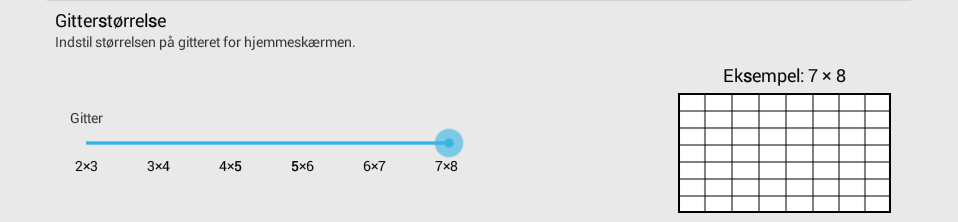
\includegraphics[width=\textwidth]{sprint_four/grid_setting_before}
        \caption{Grid setting before}
        \label{fig:launcher_grid_settings_old}
        \vspace*{1cm}
    \end{subfigure}
    \begin{subfigure}[t]{0.75\textwidth}
        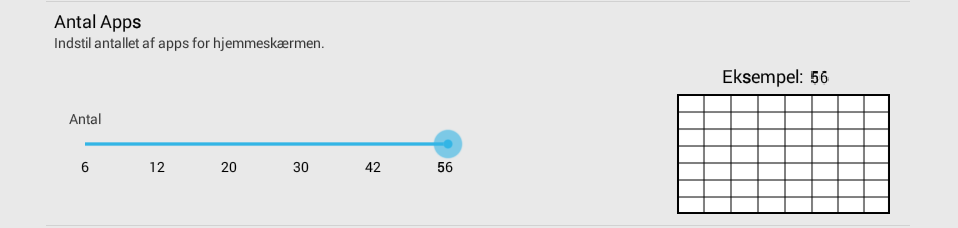
\includegraphics[width=\textwidth]{sprint_four/grid_setting_after}
        \caption{Grid setting after}
        \label{fig:launcher_grid_settings_new}
    \end{subfigure}
    
    \caption{Launcher grid settings before and after}
    \label{fig:launcher_grid_settings}
\end{figure}

%!TEX root = ../../../super_main.tex

\section{Following design guides}
\label{sec:following_design_guides}
During the fourth sprint we had a look at the applications we had been working on along with our own design guide line and we found that there were some minor problems which required our attention. Some of these problems will be described in this section.

\subsection{Wrong sidebar}
\label{sec:wrong_sidebar}
Among these minor issues we found that the side bar in the settings of the \launcher did not follow our own design guide. It did not use a proper background and did not use a \androidinline{GirafPictogramItemView} in order to display profile images. The \launcher's settings side bar, before and after, can be seen in \figref{fig:launcher_settings_side_bar_before_and_after}. Furthermore, the icons used in the side bar were also updated. The new icons can be seen in \figref{fig:launcher_settings_side_bar_after}.

\begin{figure}[!htbp]
    \centering

    \begin{subfigure}[t]{0.3\textwidth}
        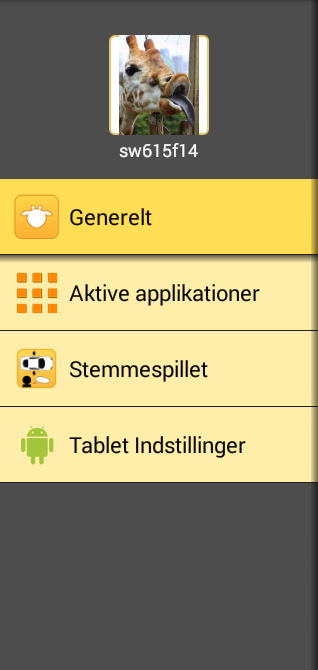
\includegraphics[width=\textwidth]{sprint_four/settings_side_bar_before}
        \caption{Before}
        \label{fig:launcher_settings_side_bar_before}
    \end{subfigure}
    \hspace{5em} 
    \begin{subfigure}[t]{0.3\textwidth}
        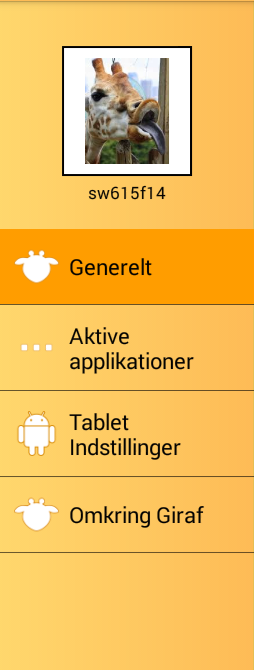
\includegraphics[width=\textwidth]{sprint_four/settings_side_bar_after}
        \caption{After}
        \label{fig:launcher_settings_side_bar_after}
    \end{subfigure}
    
    \caption{Launcher settings side bar before and after}
    \label{fig:launcher_settings_side_bar_before_and_after}
\end{figure}

%!TEX root = ../../../super_main.tex

\section{Server Issues}
\label{sec:server_issues}

The reader is invited to reference \figref{fig:bonefire} while reading this section. This is a timeline illustrating the events happened in the period with server-issues. 

\begin{figure}[!htbp]
	\centering
	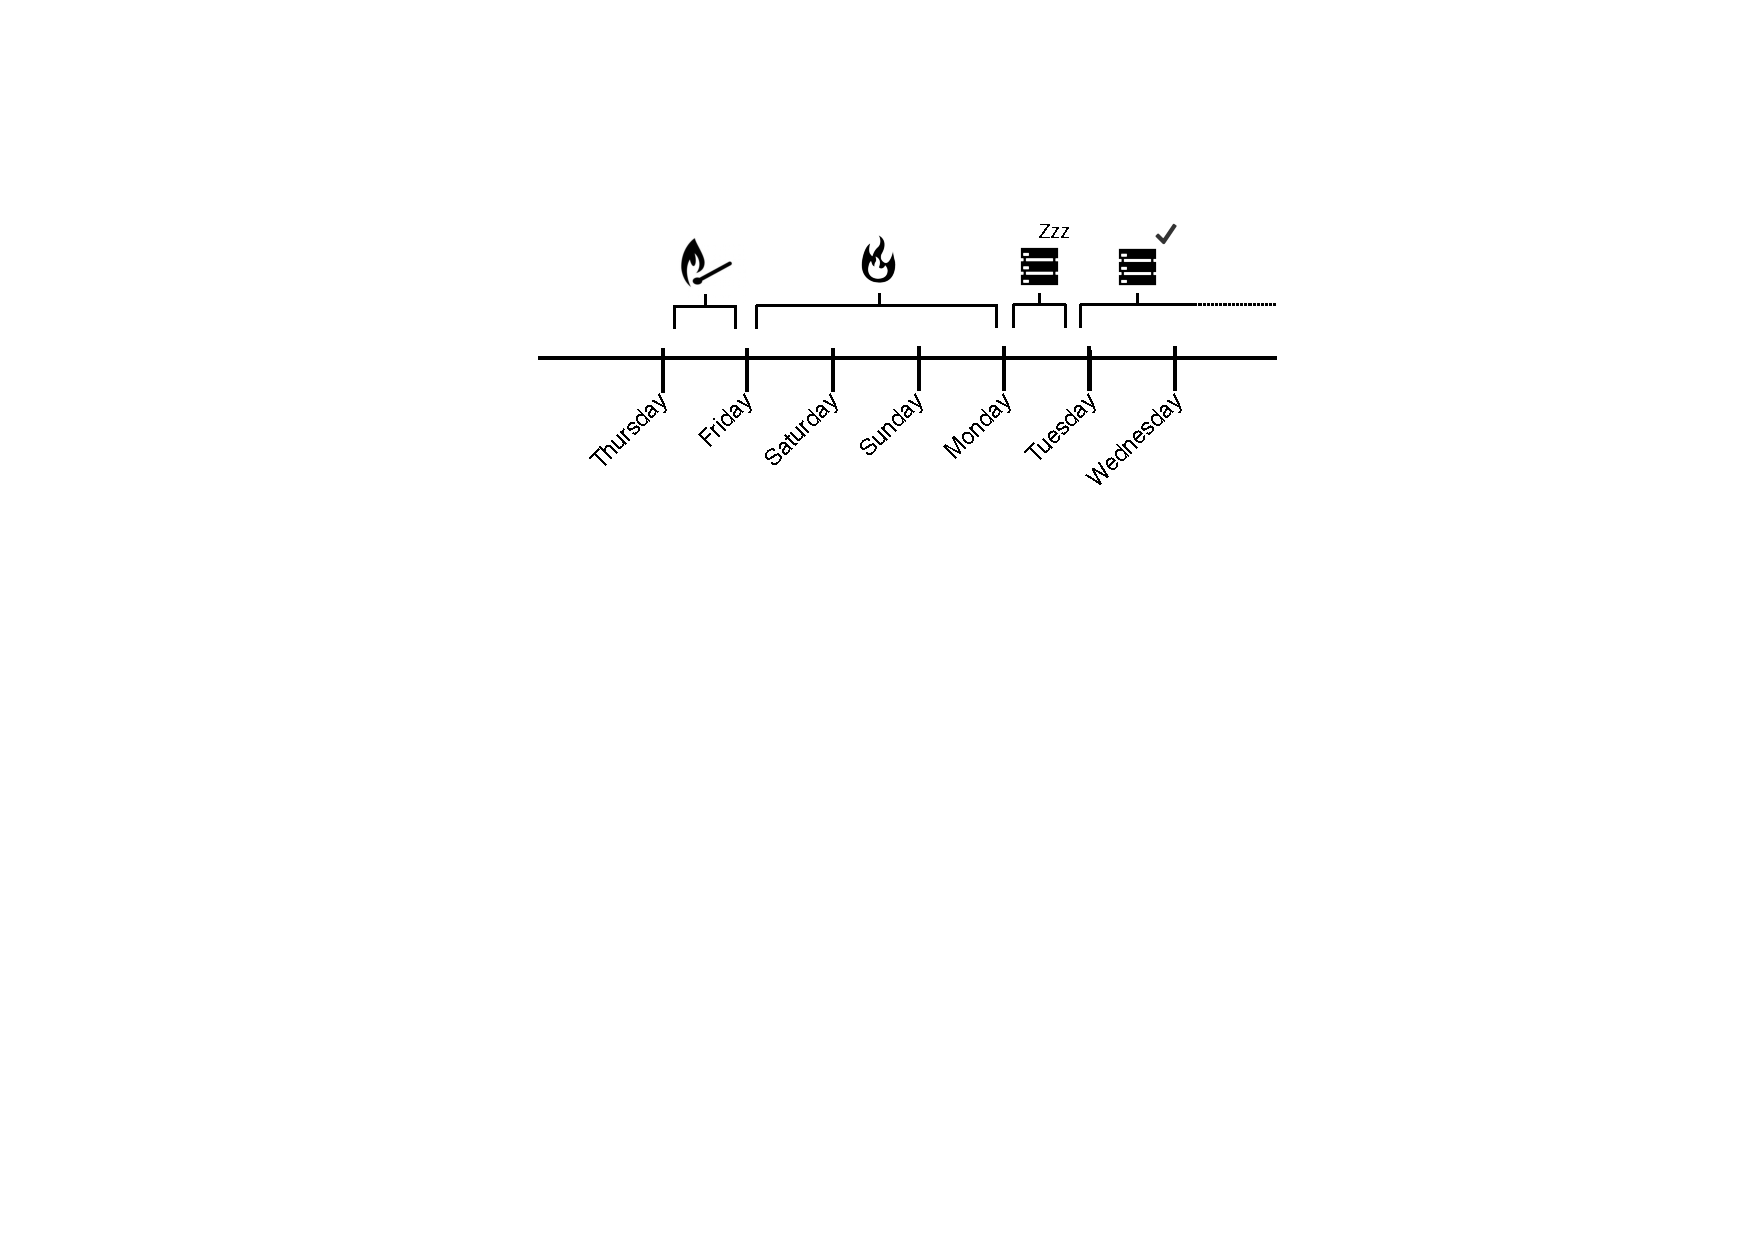
\includegraphics[width=0.75\textwidth]{bonfire}
	\caption{Timeline for the server issues}
	\label{fig:bonefire}
\end{figure}

Nearing the end of sprint four, one of the \emph{Build and Deployment} groups decided to upgrade the server with additional storage. This was attempted the night between Thursday and Friday before the planned sprint end the Wednesday after, i.e. we had five days (three actual work days and two weekend days) in between these two dates. This storage upgrade caused the entire server to crash due to some partitioning issues they had introduced. The group responsible for the update worked Friday, the entire weekend and a few hours Monday on restoring the server to a working state. Once the server worked again, the server had been rolled back to its state around 1$\frac{1}{2}$ weeks earlier, which meant that mismatches were introduced between the Git repositories located on the server and the Git repositories located on the developers' computers. 
\\\\
This resulted in having to push the different repositories to the git server again, however this was not a simple task. In order to maintain the dependencies and version numbering, we first had to sort out all dependencies between every project. Afterwards we had to locate the developers with the newest editions of the various repositories, such that we were sure that no code was lost during this process. When these people had been located, we had to make sure that the pushes were initiated in the correct order, starting from the deepest nested library, such that the development environment could be restored to its previous state correctly.
\\\\
This process was started Monday afternoon around 15:00, which is also the final obligatory working hour across the project. Therefore some people had gone home, and one library did therefore not have its newest edition uploaded to the server. This created some issues in the system which were difficult to find the cause of, since we could not possibly know that one developer had local changes that were not on the server. Our group therefore spent the entire Monday tracking down people who had information about the following issues:

\begin{enumerate}
    \item Download from remote server would not start on any client side application.
    \item Unable to login due to a ``The database does not contain any profiles'' error.
    \begin{itemize}
        \item Note: Issue 2 was revealed once issue 1 had been resolved
    \end{itemize}
    \item Unable to start applications from the \launcher  
    \begin{itemize}
        \item Note: Issue 3 was revealed once issue 2 had been resolved
    \end{itemize}
\end{enumerate}


Issue 1 was related to rolling back the MySQL server, which had created a mismatch between the MySQL user password located on the Jenkins server and the actual password needed to access the database. This was resolved due to help from group \emph{SW610F15}, whom suggested changing the MySQL password to a previous version.
\\\\
Once issue 1 had been resolved, issue 2 presented itself when trying to log into the \giraf \launcher. No matter how one attempted to login, an Android Toast (small message) would be displayed saying that no profiles were present in the database. This issue was directly related to one of the groups not pushing all their work after the server reset. This group had been working on making some applications standalone, and therefore also worked on a standalone \androidinline{ContentProvider}. A \androidinline{ContentProvider} is used in Android applications to manage access to a data source \parencite{android_content_provider}. 
\\\\
The \androidinline{ContentProvider} used by the standalone applications would change from the \androidinline{ContentProvider} provided by the \launcher to the application's own standalone \androidinline{ContentProvider}. The paths to the content provider they should use, is found in a file called \mono{QuxContentProviderAuthority.java}.
\\\\
This new way of managing content providers, unfortunately had the side effect, that the \launcher also had to have a file called \mono{QuxContentProviderAuthority.java} which had to reference its own content provider in order to make the \launcher work properly. The issue then was, that the \launcher did not have such a file, since the group working on standalone applications had not informed anyone else about how this new system worked, and the file committed by the standalone group had not been added to the \launcher repository after the rollback. 
\\\\
The effect of this missing file was that any SQL calls would just return that the size of any accessed table was zero, even though it was clearly visible through the log in Android Studio that all data was downloaded with the initial download. Once this had been discovered, the missing \mono{QuxContentProviderAuthority.java} file was added to the launcher and the login functionality was once again working.
\\\\
Hereafter it was discovered that all the other applications were getting the same error as in issue 2, once attempted launched through the \launcher application (issue 3). This was caused by a coding mistake in the \emph{Meta-Database} repository which contains the implementation of how to handle the content providers mentioned in issue 2. The implementation did not correctly check whether or not applications were launched from the \launcher, which caused every application to have to contain the \mono{QuxContentProviderAuthority.java} as well, which was not intended by the group who worked on the content providers. To solve the issue we included the Qux file in every application, and we could finally correctly start all the applications come Tuesday around 17:00. 
\\\\
We managed to solve all three issues, such that all applications in the \giraf suite was in a usable state, and we could therefore successfully execute the Sprint Review Meeting with customers present without any issues or crashes. Furthermore the group which had introduced issue 2 and 3 were aware of the mistake, and implemented a fix by Wednesday afternoon such that only the standalone applications and the \launcher were required to have the \mono{QuxContentProviderAuthority.java} file when updated to new versions of their libraries.
\\\\
Even though we managed to solve the issues after the server crash, the consequences was that there was spent a lot of time on resolving an issue rather than spending time on resolving other development tasks. Since this problem occurred so close to the end of the sprint, some groups were forced to extend the workdays to reach the goal of stable and polished applications.


%!TEX root = ../../../super_main.tex

\chapter{New Features}
\label{cha:new_features}
Additional new features have been developed in the fourth sprint. These new features will be described in this chapter.

%!TEX root = ../../../super_main.tex

\section{Bug Splash Screen}
\label{sec:bug_splash_screen}

We have implemented a bug splash screen with the hope of displaying a more meaningful and assuring message in case of uncaught exceptions rather than just letting the application crash. The bug splash screen also prints a stack trace of the GUI thread in order to help future developers whom might have forgotten to attach a debugger the one time some rare race condition occurred. An example can be seen in \figref{fig:bug_splash_screen_example}.

The bug splash screen works by setting an \androidinline{UncaughtExceptionHandler} on the shared GUI thread of an application every time a \androidinline{GirafActivity} is created. An existing \androidinline{UncaughtExceptionHandler} would simply be overridden.

\begin{figure}[!htbp]
        \centering
        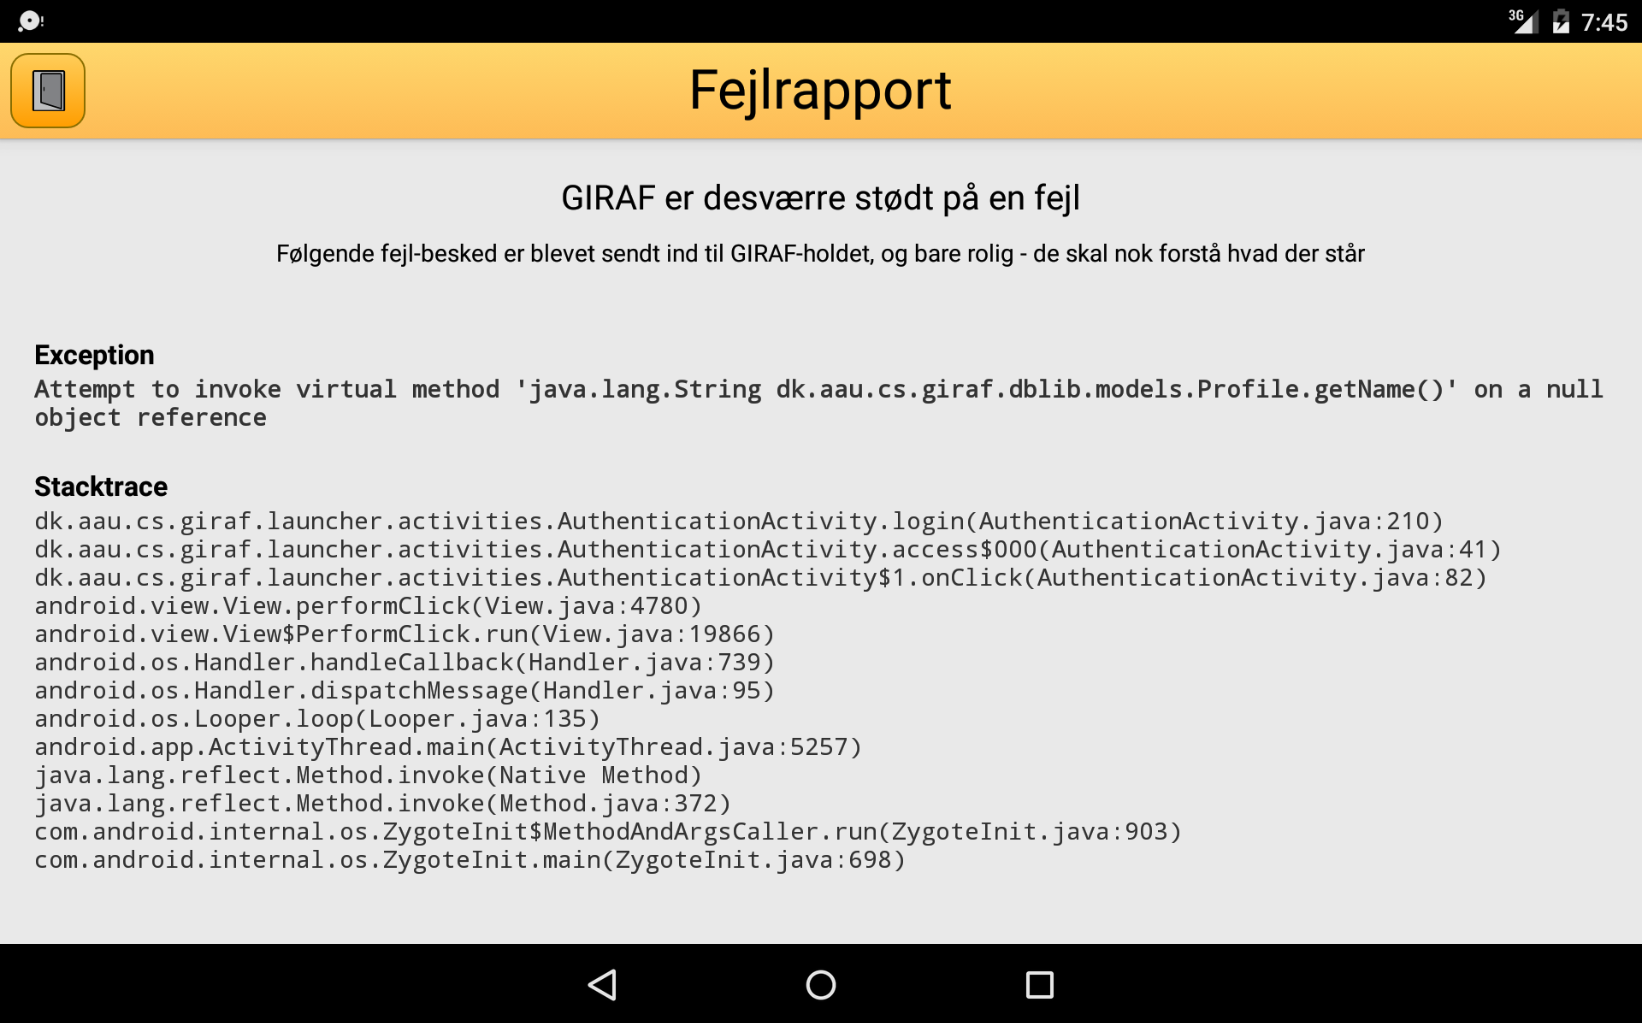
\includegraphics[width=0.75\textwidth]{sprint_four/bug_splash_screen}
        \caption{Bug splash screen example}
        \label{fig:bug_splash_screen_example}
\end{figure}

\subsection{Only GUI thread} 
The bug splash screen only works for the main thread of the application, e.i. the GUI thread, because it would be too cumbersome to apply an \androidinline{UncaughtExceptionHandler} to every new thread started. Some background threads, i.e. not the GUI thread, might be managed indirectly by the Android framework e.g. in the \androidinline{doInBackground} method of an \androidinline{AsyncTask}. We could in theory subclass \androidinline{AsyncTask} and provide an implementation of \androidinline{doInBackground} which would set an \androidinline{UncaughtExceptionHandler} on the background thread managed by the \androidinline{AsyncTask}. All uses of \androidinline{AsyncTask} across the \giraf multiproject should then change to use our new subclass of \androidinline{AsyncTask} and should then call super in their implemenation of \androidinline{doInBackground}. This would apply our bug splash screen to a significant portion all running code but would still not apply the bug splash screen to all code as there are many other ways to spawn new threads. 

We decided not to attempt to apply the bug splash screen to all threads because we anticipated that it would take too much time to implement and we did not know if it would even be possible to apply it to all thread.          


%!TEX root = ../../../super_main.tex

\section{About page}
\label{sec:about_page}

We have implemented an about page, with a simple layout, in the \launcher settings in order to properly give credit to the open source projects used in the \launcher, and thereby in the entire \giraf application suite because of the shared service provide in the \launcher. This was requested by group SW610F15 (The database subproject product owner). The about page can be seen in \figref{fig:about_page}.
\\\\
Please notice that the icon used for the about-tab could be change to something different than the general-tab, for instance an information i. However, no icons have been added for this use-case, so a last-minute solution was implemented. Ideally a new icon should be designed, implemented and described in the design manual.

\begin{figure}[!htbp]
	\centering
	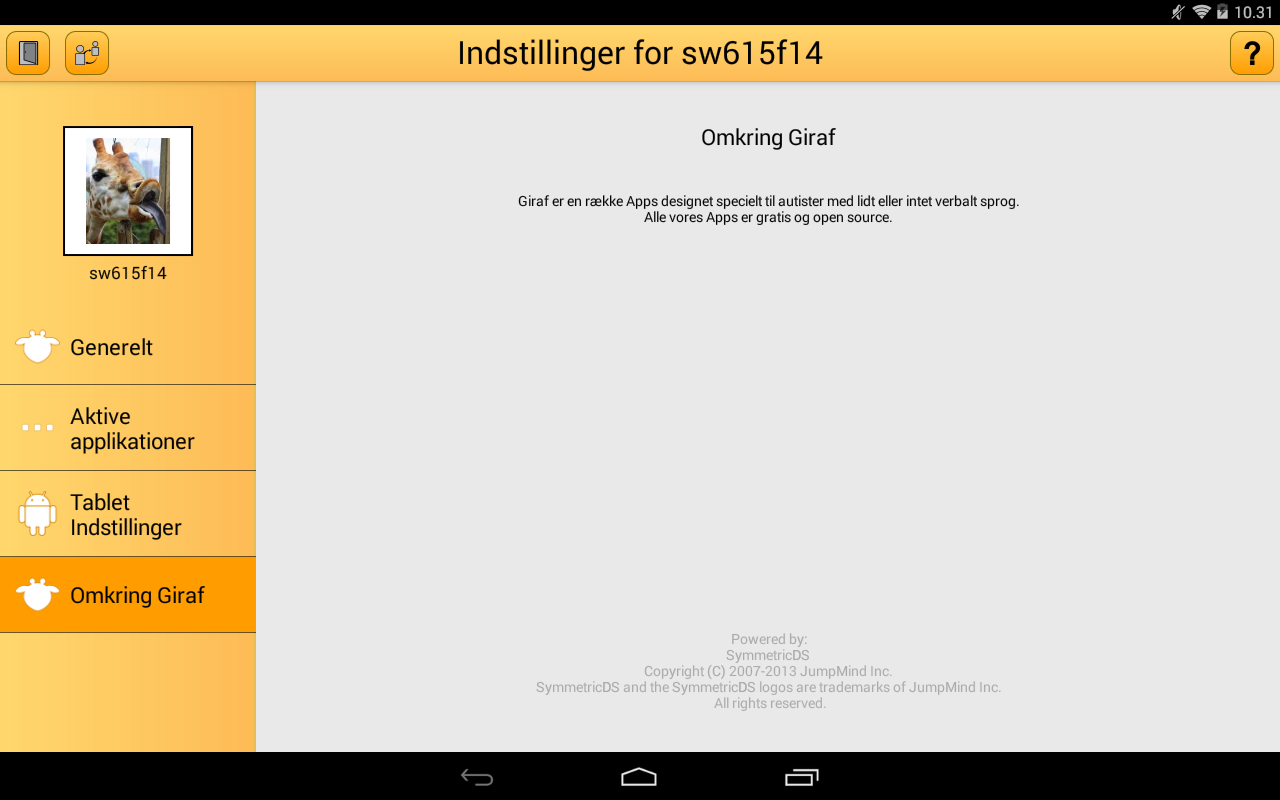
\includegraphics[width=\textwidth]{sprint_four/about_page}
	\caption{About page}
	\label{fig:about_page}
\end{figure}



%!TEX root = ../../super_main.tex

\chapter{Sprint Conclusion}
\label{cha:conclusion_sprint_4}

The fourth sprint concluded with a presentation to the customers. The two applications we had been working on, along with the other groups' applications, were presented to the customers on a big screen and the customers seemed satisfied with the development. One of the group members during the presentation can be seen in \figref{fig:sprint_review_meeting_presentation}, where he is currently presenting the final state of the \launcher 's home screen.

\begin{figure}[!htbp]
    \centering
    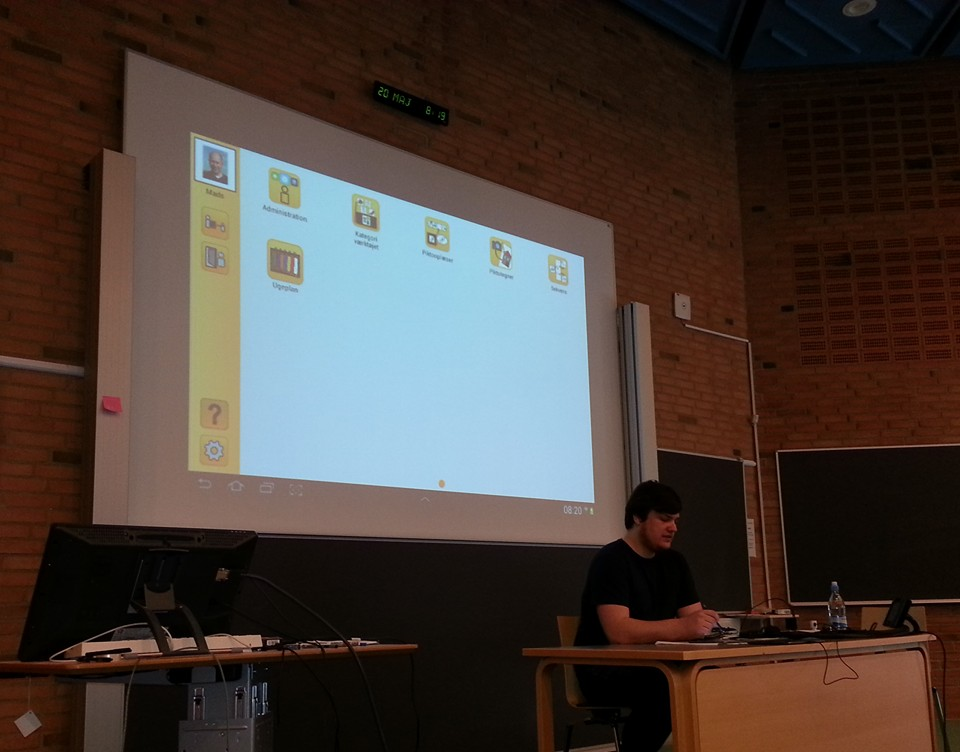
\includegraphics[width=0.75\textwidth]{sprint_four/sprint_review_meeting_presentation}
    \caption{Sprint Review Meeting Presentation}
    \label{fig:sprint_review_meeting_presentation}
\end{figure}

\FloatBarrier

The design manual was completed to a level which describes the design decisions that have been made throughout this semester. This was done in the effort to streamline the \giraf software suite. The design manual includes the design decisions that we found most important, but we have left some open problems, where we had not yet found satisfying solutions, for future \giraf developers to pursue. We encourage future \giraf developers to continue the development of this design manual on the \giraf Git server.
\\\\
In order to assist other groups, we have been actively pursuing them to confront them about not conforming to our design manual and not using the new \gc, as a part of the ``\giraf Police'' responsibility. We also provided support and updated the \gc as more people began to use them and thereby found shortcomings and bugs. 
\\\\
In the early stages of this project we were assigned the responsibility of maintaining the web page \url{www.giraf.cs.aau.dk}. However, during this semester we did not have any user stories from the customers regarding this website and have therefore not been working on it. We did though receive a request from the semester coordinator, \emph{Ulrik Nyman}, that he wanted us to update the favicon of the web page, but we never met this request because we felt that we had more important things to do.

\todo{Fjern lort fra den her part som ikke er med, evt lave en ny part der hedder Project end}